%!TEX root = ../thesis.tex
% ******************************* Thesis Appendix B ********************************

\chapter{Histograms of Time To Decision}



\begin{landscape}
\centering
\vspace*{\fill}
\begin{table}[h!]
  \centering
  \begin{tabular}{ | c | c | c | c | c |}
    \hline
    & $\epsilon$-Greedy & Sweep & Random & Saccadic \\
    \hline
    % \multicolumn{2}{c}{Initial Uniform Distribution of Belief Over Grid Cells}\\
    %\hline
    %single RAV
    %\begin{minipage}[c][height][c]{width}
    Gaussian & \vline
    \begin{minipage}[c][45mm][c]{45mm}
      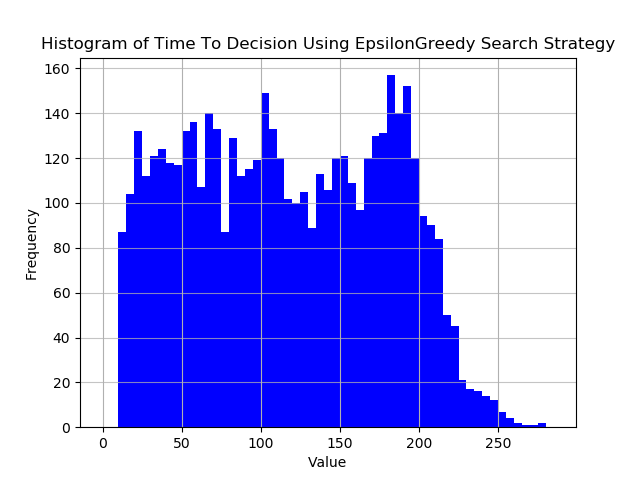
\includegraphics[width=44mm, height=44mm]{Chapters/MultiAgentTargetDetection/Figs/Results/Prior/Gaussian/SingleAgentSingleSourceGaussianEpsilonGreedyHistogram.png}
    \end{minipage}
    &
    %\hline
    %\multicolumn{2}{c}{Initial Discretised Gaussian Distribution of Belief Over Grid Cells (random mean, covariance matrix = [[], []]}\\
    %\hline
    %single RAV
    %\begin{minipage}[c][height][c]{width}
    \begin{minipage}[c][45mm][c]{45mm}
      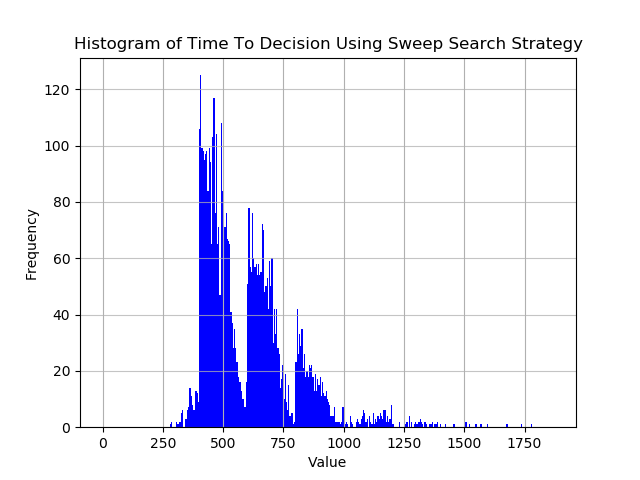
\includegraphics[width=44mm, height=44mm]{Chapters/MultiAgentTargetDetection/Figs/Results/Prior/Gaussian/SingleAgentSingleSourceGaussianSweepHistogram.png}

    \end{minipage}
    &
    \begin{minipage}[c][45mm][c]{45mm}
      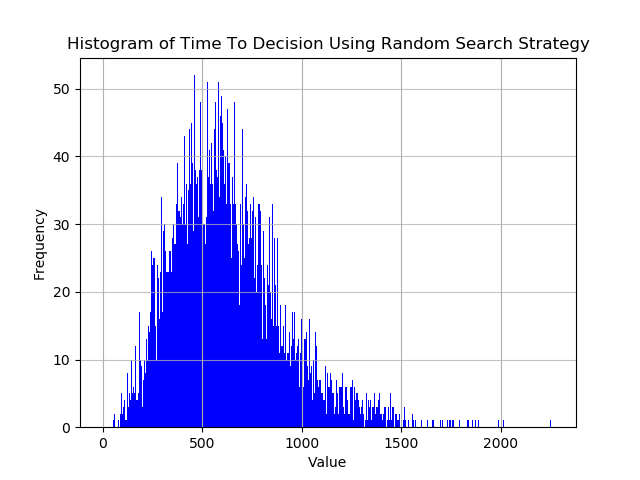
\includegraphics[width=44mm, height=44mm]{Chapters/MultiAgentTargetDetection/Figs/Results/Prior/Gaussian/SingleAgentSingleSourceGaussianRandomHistogram.png}
    \end{minipage}
    &
    \begin{minipage}[c][45mm][c]{45mm}
      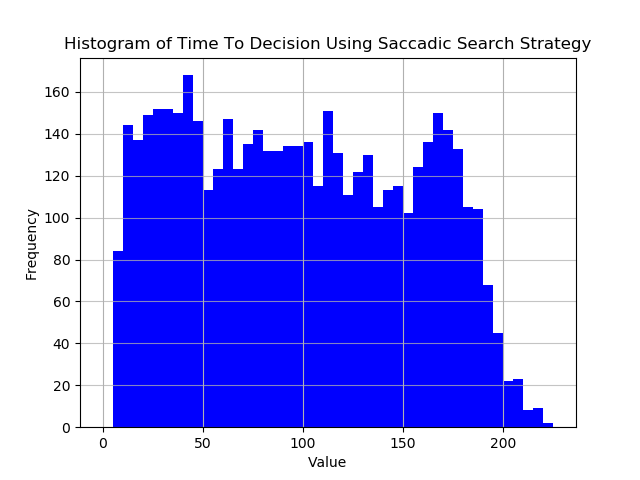
\includegraphics[width=44mm, height=44mm]{Chapters/MultiAgentTargetDetection/Figs/Results/Prior/Gaussian/SingleAgentSingleSourceGaussianSaccadicHistogram.png}
    \end{minipage}
    \\
    %&
    %\small
    %\begin{tabular}{c|c|c|c|c|c|c|c}
    %    Strategy & p(T \Romannum{1}) & p(T \Romannum{2}) & Sim. FPR & Sim. FNR & E[TTD] & Prec. & Rec \\
    %    \hline
    %    $\epsilon$ -Greedy& 4 & 2 & 0.05 & 233.2 & 2303.3 & 2 & 9\\
    %    Sweep & 4 & 2 & 0.05 & 233.2 & 2303.3 & 2 & 9\\
    %    Saccadic & 4 & 2 & 0.05 & 233.2 & 2303.3 & 2 & 9\\
    %    Random & 4 & 2 & 0.05 & 233.2 & 2303.3 & 2 & 9\\

    %\end{tabular}
    %\normalsize

    \hline
   
  \end{tabular}
  \caption{Results of running the target localisation simulation with a  uniform initial belief distribution and Gaussian initial belief distribution. p(T \Romannum{1}) = The probability of making a type \Romannum{1} error using the SPRT, p(T \Romannum{2}) = The probability of making a type \Romannum{1} error using the SPRT, Sim. FPR = The simulated false positive rate of the sensor, Sim. FNR = The simulated false negative rate of the sensor, E[TTD] = The expected amount of timesteps until a decision is made, Prec. = precision, Rec. = Recall. }\label{table:ORToolsResults}
\end{table}
\end{landscape}
